\documentclass{article}
\usepackage{amsmath}
\usepackage{listings}
\usepackage{xcolor}
\usepackage{graphicx}

\definecolor{codegreen}{rgb}{0,0.6,0}
\definecolor{codegray}{rgb}{0.5,0.5,0.5}
\definecolor{codepurple}{rgb}{0.58,0,0.82}
\definecolor{backcolour}{rgb}{0.95,0.95,0.92}

\lstdefinestyle{mystyle}{
    backgroundcolor=\color{backcolour},   
    commentstyle=\color{codegreen},
    keywordstyle=\color{magenta},
    numberstyle=\tiny\color{codegray},
    stringstyle=\color{codepurple},
    basicstyle=\ttfamily\footnotesize,
    breakatwhitespace=false,         
    breaklines=true,                 
    captionpos=b,                    
    keepspaces=true,                 
    numbers=left,                    
    numbersep=5pt,                  
    showspaces=false,                
    showstringspaces=false,
    showtabs=false,                  
    tabsize=2
}

\lstset{style=mystyle}
\begin{document}


\noindent
\textbf{20170082 Dongwon Kim EE412 HW\#2}\\

\section*{1}
\subsection*{1-(a)}
Suppose the set is $S = \{a, aa, aaaa, aaaaaaaa, aaaaaaaaaaaaaaaa\}$
Then the editdistance for each element to the rest of the element is:
\begin{align*}
    &editdistance(a, aa) = 1 \\
    &editdistance(a, aaaa) = 3 \\
    &editdistance(a, aaaaaaaa) = 7 \\
    &editdistance(a, aaaaaaaaaaaaaaaa) = 15 \\
    &editdistance(aa, aaaa) = 2 \\
    &editdistance(aa, aaaaaaaa) = 6 \\
    &editdistance(aa, aaaaaaaaaaaaaaaa) = 14 \\
    &editdistance(aaaa, aaaaaaaa) = 4 \\
    &editdistance(aaaa, aaaaaaaaaaaaaaaa) = 12 \\
    &editdistance(aaaaaaaa, aaaaaaaaaaaaaaaa) = 8 \\
\end{align*}
So the sum of the editdistance for each element is,
\begin{align*}
    a &\rightarrow 1 + 3 + 7 + 15 = 26 \\
    aa &\rightarrow 1 + 2 + 6 + 14 = 23 \\
    aaaa &\rightarrow 3 + 2 + 4 + 12 = 21 \\
    aaaaaaaa &\rightarrow 7 + 6 + 4 + 8 = 25 \\
    aaaaaaaaaaaaaaaa &\rightarrow 15 + 14 + 12 + 8 = 49 \\
\end{align*}
Where the clustroid becomes aaaa with the minimum sum of editdistance, 21.
The maximum of the editdistance for each element is,
\begin{align*}
    a &\rightarrow 15 \\
    aa &\rightarrow 14 \\
    aaaa &\rightarrow 12 \\
    aaaaaaaa &\rightarrow 8 \\
    aaaaaaaaaaaaaaaa &\rightarrow 15 \\
\end{align*}
Where the clustroid becomes aaaaaaaa with the minimum of 15.


\subsection*{1-(b)}
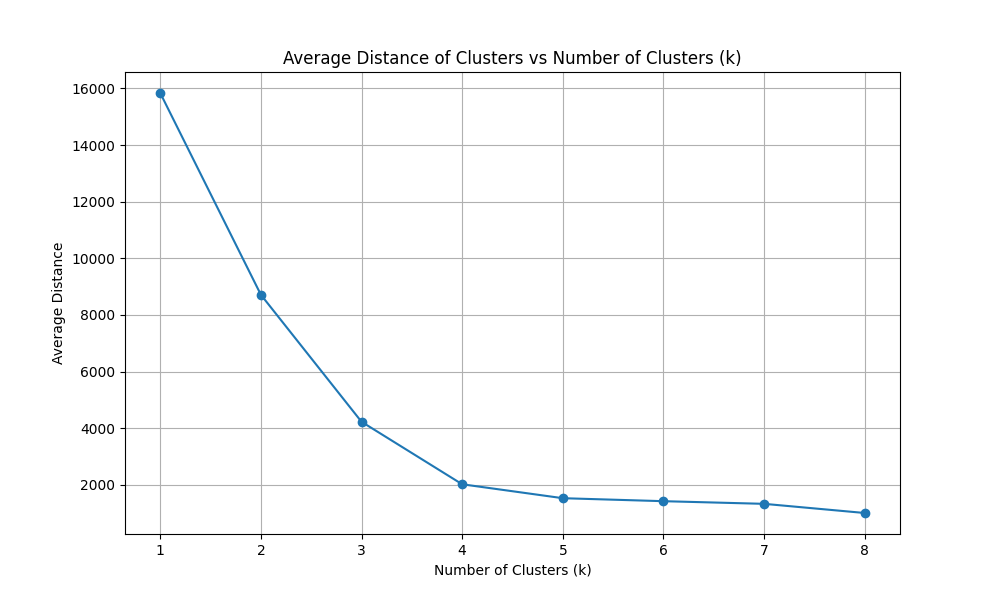
\includegraphics[scale=0.4]{cluster_plot.png}\\
The k value with an explanation why it is good for this data.
The answer is 5, as the difference between the average distance begins to decrease insignificantly (i.e. smaller than 10\%) after k = 5.
The difference is over 10\% in case of k = 8, but this requires more clusters, increasing model complexity.
If higher complexity (i.e. more clusters) is desirable, then k = 8 is also a good choice.

\section*{2}
\subsection*{11.1.7}
Following is the code for the problem.

\begin{lstlisting}[language=Python]
    import numpy as np


    def power_iteration(A, B, nsim):
        # Choose a random starting vector
        b_k = B
    
        for _ in range(nsim):
            # Calculate the matrix-by-vector product Ab
            b_k1 = np.dot(A, b_k)
    
            # Re normalize the vector
            b_k = b_k1 / np.linalg.norm(b_k1)
    
        return b_k
    
    
    def main():
        A = np.array([[1, 1, 1], [1, 2, 3], [1, 3, 6]])
        B = np.array([1, 1, 1])
    
        eigvec = power_iteration(A, B, nsim=100)
        eigval = np.dot(np.dot(A, eigvec), eigvec)
    
        print("eigvec: ", np.around(eigvec, decimals=3))
        print("eigval: ", np.around(eigval, decimals=3))
    
        # second eigenvalue
        A1 = A - eigval * np.outer(eigvec, eigvec)
        print("A: ", np.around(A1, decimals=3))
    
        eigvec = power_iteration(A1, B, nsim=100)
        eigval = np.dot(np.dot(A1, eigvec), eigvec)
    
        print("eigvec: ", np.around(eigvec, decimals=3))
        print("eigval: ", np.around(eigval, decimals=3))
    
        # third eigenvalue
        A2 = A1 - eigval * np.outer(eigvec, eigvec)
        print("A: ", np.around(A2, decimals=3))
    
        eigvec = power_iteration(A2, B, nsim=100)
        eigval = np.dot(np.dot(A2, eigvec), eigvec)
    
        print("eigvec: ", np.around(eigvec, decimals=3))
        print("eigval: ", np.around(eigval, decimals=3))
    
    
    if __name__ == "__main__":
        main()    
\end{lstlisting}

The result for the problem is as follows.

\begin{enumerate}
    \item [(a)] $\begin{bmatrix} 0.194 \\ 0.472 \\ 0.86 \\  \end{bmatrix}$
    \item [(b)] $7.873$
    \item [(c)] 
    $A = \begin{bmatrix}
            0.704 & 0.279 & -0.312 \\
            0.279 & 0.244 & -0.197 \\
            -0.312 & -0.197 & 0.179 \\            
    \end{bmatrix}$
    \\
    \item [(d)] $\begin{bmatrix}  0.816 \\  0.408 \\ -0.408 \\ \end{bmatrix}, 1.0$
    \item [(e)]
    $A = \begin{bmatrix} 
            0.038 & -0.054 & 0.021 \\
            -0.054 & 0.078 & -0.03 \\
            0.021 & -0.03 & 0.012 \\
    \end{bmatrix}$ \\
    \\
    eigvec: $\begin{bmatrix} 0.544 \\ -0.781 \\ 0.306 \\ \end{bmatrix}$ \\
    \\
    eigval: $0.127$
\end{enumerate}

\subsection*{11.1.7}
Following is the code for the problem.

\begin{lstlisting}[language=Python]
import numpy as np

def main():
    M = [[1, 2, 3], [3, 4, 5], [5, 4, 3], [0, 2, 4], [1, 3, 5]]
    M = np.array(M)
    transpose_M = np.transpose(M)

    MtM = np.matmul(transpose_M, M)
    print("transpose(M)*M:")
    print(MtM)

    MMt = np.matmul(M, transpose_M)
    print("M*transpose(M):")
    print(MMt)

    # Find eigenpairs
    eigval_MtM, eigvec_MtM = np.linalg.eig(MtM)
    # sort eigenpairs
    idx = eigval_MtM.argsort()[::-1]
    eigval_MtM = eigval_MtM[idx]
    eigvec_MtM = eigvec_MtM[:, idx]

    eigval_MMt, eigvec_MMt = np.linalg.eig(MMt)
    # sort eigenpairs
    idx = eigval_MMt.argsort()[::-1]
    eigval_MMt = eigval_MMt[idx]
    eigvec_MMt = eigvec_MMt[:, idx]

    print("Eigenvalues of Transpose(M)*M:")
    print(np.around(eigval_MtM, decimals=3))
    print("Eigenvectors of Transpose(M)*M:")
    print(np.around(eigvec_MtM, decimals=3))

    print("Eigenvalues of M*Transpose(M):")
    print(np.around(eigval_MMt, decimals=3))
    print("Eigenvectors of M*Transpose(M):")
    print(np.around(eigvec_MMt, decimals=3))

    # find SVD using above only two eigenpairs
    V = eigvec_MtM[:, :2]
    S = np.sqrt(np.diag(eigval_MtM[:2]))

    # calculate U using V and S
    U = np.matmul(np.matmul(M, V), np.linalg.inv(S))

    print("U:")
    print(np.around(U, decimals=3))
    print("S:")
    print(np.around(S, decimals=3))
    print("V:")
    print(np.around(V, decimals=3))
    print("U*S*V^T:")
    print(np.around(np.matmul(np.matmul(U, S), V.T), decimals=3))
    print("M:")
    print(np.around(M, decimals=3))

    # rank 1 approximation
    U1 = U[:, :1]
    S1 = S[:1, :1]
    V1 = V[:, :1]
    M1 = np.matmul(np.matmul(U1, S1), V1.T)
    print("rank 1 approximation of M:")
    print(np.around(M1, decimals=3))

    print("energy of the original singular values:")
    print(np.around(np.sum(S**2), decimals=3))
    print("energy of the one-dimensional approximation:")
    print(np.around(np.sum(S1**2), decimals=3))


if __name__ == "__main__":
    main()

\end{lstlisting}

The result for the problem is as follows.
\begin{enumerate}
    \item[(a)] The matrices \( M^T M \) and \( M M^T \) are given by:\\
    \[
    M^T M = \begin{bmatrix}
        36 & 37 & 38 \\
        37 & 49 & 61 \\
        38 & 61 & 84
    \end{bmatrix}
    \]
    and
    \[
    M M^T = \begin{bmatrix}
        14 & 26 & 22 & 16 & 22 \\
        26 & 50 & 46 & 28 & 40 \\
        22 & 46 & 50 & 20 & 32 \\
        16 & 28 & 20 & 20 & 26 \\
        22 & 40 & 32 & 26 & 35
    \end{bmatrix}
    \]

    \item[(b)] The eigenpairs for the matrices \( M^T M \) and \( M M^T \) are:\\
    \\
    For \( M^T M \):\\
    \\
    Eigenvalues: \( [153.567,  15.433,   0.0] \)\\
    Eigenvectors:
    \[
    \begin{bmatrix}
        -0.409 & -0.816 & 0.408 \\
        -0.563 & -0.126 & -0.816 \\
        -0.718 & 0.564  & 0.408
    \end{bmatrix}
    \]
    For \( M M^T \):\\
    \\
    Eigenvalues: \( [153.567,  15.433,   0.0,   -0.0,   -0.0] \)\\
    Eigenvectors:
    \[
    \begin{bmatrix}
     0.298 & -0.159 & 0.125 & 0.075 & 0.941 \\
    0.571 & 0.033 & -0.453 & -0.073 & -0.175 \\
    0.521 & 0.736 & 0.326 & -0.106 & -0.04 \\
    0.323 & -0.51 & 0.72  & -0.726 & -0.188 \\
    0.459 & -0.414 & -0.393 & 0.672 & -0.215
    \end{bmatrix}
    \]

    \item[(c)] The Singular Value Decomposition (SVD) for the matrix \( M \) is:\\
    \( U \):
    \[
    \begin{bmatrix}
        -0.298 & 0.159 \\
        -0.571 & -0.033 \\
        -0.521 & -0.736 \\
        -0.323 & 0.51 \\
        -0.459 & 0.414
    \end{bmatrix}
    \]
    \( \Sigma \):
    \[
    \begin{bmatrix}
        12.392 & 0 \\
        0 & 3.928
    \end{bmatrix}
    \]
    \( V \):
    \[
    \begin{bmatrix}
        -0.409 & -0.816 \\
        -0.563 & -0.126 \\
        -0.718 & 0.564
    \end{bmatrix}
    \]

    \item[(d)] The one-dimensional approximation to the matrix \( M \) is:
    \[
    \begin{bmatrix}
        1.51 & 2.079 & 2.647 \\
        2.894 & 3.984 & 5.074 \\
        2.641 & 3.636 & 4.631 \\
        1.636 & 2.252 & 2.869 \\
        2.328 & 3.205 & 4.082
    \end{bmatrix}
    \]

    \item[(e)] The energy of the original singular values is \( 169.0 \). The energy of the one-dimensional approximation is \( 153.567 \). The fraction of energy retained is given by the ratio of the energy of the approximation to the original energy.
\end{enumerate}

\subsection*{3-(a)}

\subsection*{9.3.1}
\begin{enumerate}
    \item[(a)]
            \[
            \begin{array}{c|cccccccc}
            & a & b & c & d & e & f & g & h \\
            \hline
            A & 1 & 1 & 0 & 1 & 1 & 0 & 1 & 1 \\
            B & 0 & 1 & 1 & 1 & 1 & 1 & 1 & 0 \\
            C & 1 & 0 & 1 & 1 & 0 & 1 & 1 & 1 \\
            \end{array}
            \]
            \[
        D_J(A,B) = 1 - \frac{|A \cap B|}{|A \cup B|}
        \]

        Computing for each pair:\\

        \(D_J(A,B) = 1 - \frac{4}{8} = \frac{1}{2}\)

        \(D_J(A,C) = 1 - \frac{4}{8} = \frac{1}{2}\)

        \(D_J(B,C) = 1 - \frac{4}{8} = \frac{1}{2}\)
    \item[(b)]
        Cosine distance is given by:\\

        \[
        D_C(A,B) = acos(\frac{A \cdot B}{\|A\| \|B\|})
        \]

        Computing for each pair:\\

        \(D_C(A,B) = acos(\frac{4}{6}) = 0.841\)

        \(D_C(A,C) = acos(\frac{4}{6}) = 0.841\)

        \(D_C(B,C) = acos(\frac{4}{6}) = 0.841\)
    \item[(c)]
        \[
        \begin{array}{c|cccccccc}
        & a & b & c & d & e & f & g & h \\
        \hline
        A & 1 & 1 & 0 & 1 & 0 & 0 & 1 & 0 \\
        B & 0 & 1 & 1 & 1 & 0 & 0 & 0 & 0 \\
        C & 0 & 0 & 0 & 1 & 0 & 1 & 1 & 1 \\
        \end{array}
        \]
    
        \(D_J(A,B) = 1 - \frac{2}{5} = \frac{3}{5}\)

        \(D_J(A,C) = 1 - \frac{2}{6} = \frac{2}{3}\)

        \(D_J(B,C) = 1 - \frac{1}{6} = \frac{5}{6}\)
    \item[(d)]

        \(D_C(A,B) = acos(\frac{2}{2\sqrt{3}}) = 0.955\)

        \(D_C(A,C) = acos(\frac{2}{4}) = 1.047\)

        \(D_C(B,C) = acos(\frac{1}{2\sqrt{3}}) = 1.278\)
    
    \item[(e)]
        \( AVG(A) = (4+5+5+1+3+2)/6 = 20/6 = 10/3 \) \\
        \( AVG(B) = (3+4+3+1+2+1)/6 = 14/6 = 7/3\) \\
        \( AVG(C) = (2+1+3+4+5+3)/6 = 18/6 = 3\) \\

        The utility matrix becomes:
        \[
        \begin{array}{c|cccccccc}
        & a & b & c & d & e & f & g & h \\
        \hline
        A & 2/3 & 5/3 & 0 & 5/3 & -7/3 & 0 & -1/3 & -4/3 \\
        B & 0 & 2/3 & 5/3 & 2/3 & -4/3 & -1/3 & -4/3 & 0 \\
        C & -1 & 0 & -2 & 0 & 0 & 1 & 2 & 0\\
        \end{array}
        \]
    \item[(f)]

    \(D_C(A,B) = acos(\frac{52/9}{\sqrt{120/9}\sqrt{66/9}}) =  0.9468 \) \\
    \(D_C(A,C) = acos(\frac{-4/3}{\sqrt{120/9}\sqrt{10}}) = 1.687 \) \\
    \(D_C(B,C) = acos(\frac{-19/3}{\sqrt{66/9}\sqrt{10}}) = 2.403 \)

\end{enumerate}


\subsection*{9.3.2}
\begin{enumerate}
    \item[(a)]
    The utility matrix becomes,\\
    \[
    \begin{array}{c|cccccccc}
    & a & b & c & d & e & f & g & h \\
    \hline
    A & 1 & 1 & 0 & 1 & 0 & 0 & 1 & 0 \\
    B & 0 & 1 & 1 & 1 & 0 & 0 & 0 & 0 \\
    C & 0 & 0 & 0 & 1 & 0 & 1 & 1 & 1 \\
    \end{array}
    \]
    The smallest Jaccard distance is between f and h, whose distance is 0. So the first cluster is \{f, h\}.\\
    The second smallest is between b and d, whose distance is 1/3, so the second cluster is \{b, d\}.\\
    The third smallest is between \{b, d\} and g, whose distance is 1/3, so the third cluster is \{b, d, g\}.\\
    The fourth smallest is between \{b, d, g\} and c, whose distance is 1/2, so the fourth cluster is \{b, c, d, g\}.\\
    Therefore, the final clusters are \{a\}, \{e\}, \{f, h\}, \{b, c, d, g\}.
    \item[(b)]
    For user A, the average of \{f, h\} is 2,
    the average of \{b, c, d, g\} is 13/3.
    For user B, the average of \{f, h\} is 2,
    the average of \{b, c, d, g\} is 11/3.
    For user C, the average of \{f, h\} is 7/2,
    the average of \{b, c, d, g\} is 3.
    The utility matrix becomes,\\
    \[
    \begin{array}{c|cccccccc}
    & \{a\} & \{e\} & \{f, h\} & \{b, c, d, g\}\\
    \hline
    A & 4 & 1 & 2 & 13/3 \\
    B & null & 1 & 2 & 11/3 \\
    C & 2 & null & 7/2 & 3 \\
    \end{array}
    \]
    
    \item[(c)]
    Considering null is 0, we have,\\
    \(D_C(A,B) = acos(\frac{188/9}{\sqrt{358/9}\sqrt{166/9}}) = 0.690\)\\
    \(D_C(B,C) = acos(\frac{18}{\sqrt{166/9}\sqrt{101/4}}) = 0.584\)\\
    \(D_C(C,A) = acos(\frac{28}{\sqrt{101/4}\sqrt{358/9}}) = 0.487\)
    

\end{enumerate}


\end{document}